% Author: Joshua Payne
\documentclass[letterpaper]{article}
\usepackage[landscape]{geometry}


\usepackage[usenames,dvipsnames]{xcolor}
\usepackage{tikz}


\usepackage{ifthen}
\usetikzlibrary{chains,fit,shapes}
\usetikzlibrary{calc}

\newcommand\loopbracket[4]{% a, b, width
  
  \draw[color=#4] let \p1=(#1.west), \p2=(#2.west) in ($(\x1,\y1)$) -- ($(\x1-#3,\y1)$) -- ($(\x1-#3,\y2)$) -- ($(\x1,\y2)$);

}
\newcommand\printarray[3]{
  \begin{scope}[start chain=1 going right,node distance=0.0cm]
    \node[on chain=1,xshift=-1cm,tmtape1] at (stat#1) {};
    
    \foreach \j in #2
    {
      \node[on chain=1,tmtape1] (n#1\j) {$\j$#3};
    }
    \end{scope}
}

\begin{document}



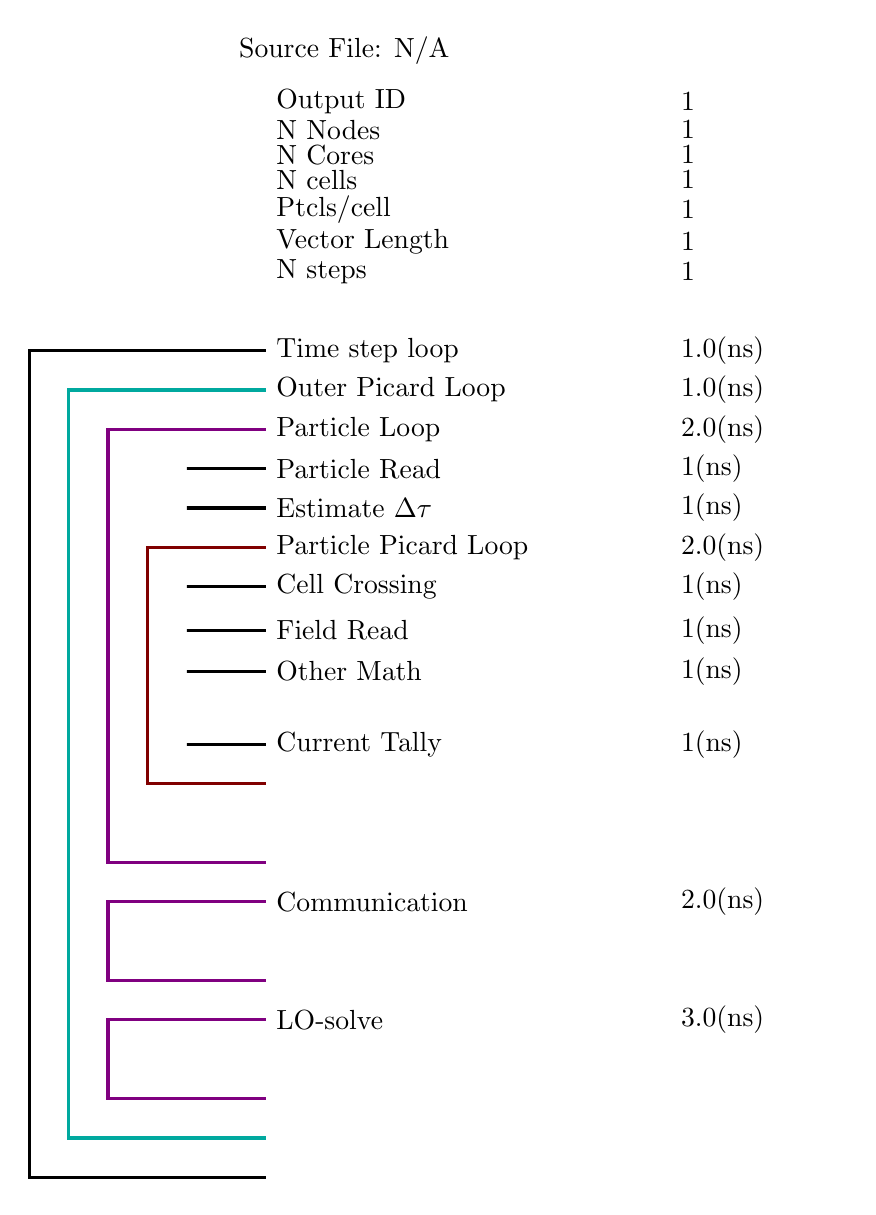
\begin{tikzpicture}
		\tikzstyle{every path}=[very thick]
		\tikzstyle{MainSty}=[->,dashdotted]
		\tikzstyle{CollSty}=[->,color=Emerald,densely dashdotted]
		\tikzstyle{ReinSty}=[->,color=Maroon,dashed]

		\edef\sizetape{1.0cm}
		\tikzstyle{tmtape}=[ text width=4cm,
				      align=left]
		\tikzstyle{tmtape1}=[ text width=2cm,
				      align=left]
\def\SourceFile{N/A}
\def\ArrayA{1.0}
\def\ArrayB{1.0}
\def\ArrayC{2.0}
\def\ArrayD{2.0}
\def\ArrayE{2.0}
\def\ArrayF{3.0}
\def\ArrayAccel{1}
\def\ArrayCurrent{1}
\def\ArrayCrossing{1}
\def\ArrayDtauEst{1}
\def\ArrayPRead{1}
\def\ArrayPOther{1}

\def\ArrayNStep{1}
\def\ArrayNX{1}
\def\ArrayNCore{1}
\def\ArrayNNode{1}
\def\ArrayNptcls{1}
\def\ArrayID{1}
\def\ArrayVecL{1}

\newcommand*{\pshiftmm}{(-2.0mm,-2.0mm)}
\newcommand*{\pshiftpm}{(2.0mm,-2.0mm)}
\newcommand*{\pshiftmp}{(-2.0mm,2.0mm)}
\newcommand*{\pshiftpp}{(2.0mm,2.0mm)}




\node[tmtape] (tstep_loop) {Time step loop};
\node[tmtape,yshift=-5mm] at (tstep_loop) (opiccard) {Outer Picard Loop};
\node[tmtape,yshift=-5mm] at (opiccard) (subcycle) {Particle Loop};
\node[tmtape,yshift=-5mm] at (subcycle) (pread) {Particle Read};
\node[tmtape,yshift=-1cm] at (pread) (ppiccard) {Particle Picard Loop};
\node[tmtape,yshift=-4.5cm] at (ppiccard) (communication) {Communication};
\node[tmtape,yshift=-1.5cm] at (communication) (solve) {LO-solve}; 

\node[tmtape,yshift=-1cm] at (solve) (solve_end) {};
\node[tmtape,yshift=-5mm] at (solve_end) (opiccard_end) {};
\node[tmtape,yshift=-5mm] at (opiccard_end) (tstep_end) {};
\node[tmtape,yshift=5mm] at (solve) (comm_end) {};
\node[tmtape,yshift=5mm] at (communication) (subcycle_end) {};
\node[tmtape,yshift=1cm] at (subcycle_end) (ppiccard_end) {};

\loopbracket{tstep_loop}{tstep_end}{3cm}{Black}
\loopbracket{solve}{solve_end}{2.0cm}{Purple}
\loopbracket{communication}{comm_end}{2.0cm}{Purple}
\loopbracket{opiccard}{opiccard_end}{2.5cm}{Emerald}
\loopbracket{subcycle}{subcycle_end}{2.0cm}{Purple}
\loopbracket{ppiccard}{ppiccard_end}{1.5cm}{Maroon}


\node[xshift=5cm] at (tstep_loop.west) (stat7) {};
\node[xshift=5cm] at (opiccard.west) (stat8) {};
\node[xshift=5cm] at (subcycle.west) (stat9) {};
\node[xshift=5cm] at (ppiccard.west) (stat10) {};
\node[xshift=5cm] at (communication.west) (stat11) {};
\node[xshift=5cm] at (solve.west) (stat12) {};

\node[tmtape,yshift=-5mm] at (pread) (statl13) {Estimate $\Delta\tau$};

\begin{scope}[start chain=1 going below,node distance=0mm]
  \node[on chain=1,tmtape,yshift=-5mm] at (ppiccard) (statl14) {Cell Crossing};
  \node[on chain=1,tmtape] (statl15) {Field Read};
  \node[on chain=1,tmtape] (statl18) {Other Math};
\end{scope}

 \node[tmtape,yshift=5mm] at (ppiccard_end) (statl16) {Current Tally};
 \node[tmtape] at (pread) (statl17) {};
  
 \foreach \i in {13,...,18}
 {
    \loopbracket{statl\i}{statl\i}{1.0cm}{Black}
    \node[xshift=5cm] at (statl\i.west) (stat\i) {};
 }
 
 

\begin{scope}[start chain=1 going above,node distance=-0.2cm]
  \node[yshift=1cm,on chain=1,tmtape] at  (tstep_loop) (statl1) {N steps};
  \node[on chain=1,tmtape] (statl30) {Vector Length};
  \node[on chain=1,tmtape] (statl5) {Ptcls/cell};
  \node[on chain=1,tmtape] (statl2) {N cells};
  \node[on chain=1,tmtape] (statl3) {N Cores};
  \node[on chain=1,tmtape] (statl4) {N Nodes};
  \node[on chain=1,tmtape] (statl6) {Output ID};
  
\end{scope}

\foreach \i in {1,...,6}
{
  \node[xshift=5cm] at (statl\i.west) (stat\i) {}; 
}

\node[xshift=5cm] at (statl30.west) (stat30) {}; 

\printarray{1}{\ArrayNStep}{}
\printarray{2}{\ArrayNX}{}
\printarray{3}{\ArrayNCore}{}
\printarray{4}{\ArrayNNode}{}
\printarray{5}{\ArrayNptcls}{}
\printarray{6}{\ArrayID}{}
\printarray{7}{\ArrayA}{(ns)}
\printarray{8}{\ArrayB}{(ns)}
\printarray{9}{\ArrayC}{(ns)}
\printarray{10}{\ArrayD}{(ns)}
\printarray{11}{\ArrayE}{(ns)}
\printarray{12}{\ArrayF}{(ns)}
\printarray{15}{\ArrayAccel}{(ns)}
\printarray{16}{\ArrayCurrent}{(ns)}
\printarray{14}{\ArrayCrossing}{(ns)}
\printarray{13}{\ArrayDtauEst}{(ns)}
\printarray{17}{\ArrayPRead}{(ns)}
\printarray{18}{\ArrayPOther}{(ns)}

\printarray{30}{\ArrayVecL}{}


\node[yshift=1cm,xshift=-4cm] at (stat4) {Source File: \SourceFile};

\end{tikzpicture}
\end{document}

